\mysection{Results}\label{sec:results}
The described method has been applied to two translational modes simultaneously. The applied feedback signal is a phase shifted version of the measured signal, with a variable gain. The use of the lock-in amplifier ensures that we send a narrow band version of the measured signal, which is difficult with analogue band pass filters. The measured lock-in signal is Fourier transformed using the Welch method, to average over the measurement time. Finally, the bandpass filter of the lock-in is compensated numerically.

The results for mode 3 and mode 4 are plotted in separate figures. In the legend, the values of the achieved mode temperatures with corresponding RMS amplitude and proportional gain are given. Increasing the proportional gain results in lowering the peak, leading to an effective broadening of the peak, as expected. Same colors in the legends of Fig.~\ref{fig:cooling3} and Fig.~\ref{fig:cooling4} correspond to the same moment in time. 

Mode 3 has a resonance frequency of \SI{50.59}{Hz} and a Q factor of \SI{3.8e6}{}. The lowest observed mode temperature for mode 3 is \SI{7.1}{mK}, obtained using a gain of \SI{930}{} and has a corresponding RMS amplitude of \SI{1.6}{pm}. %, see Fig.~\ref{fig:cooling3}.

\begin{figure}[h!]
    \centering
    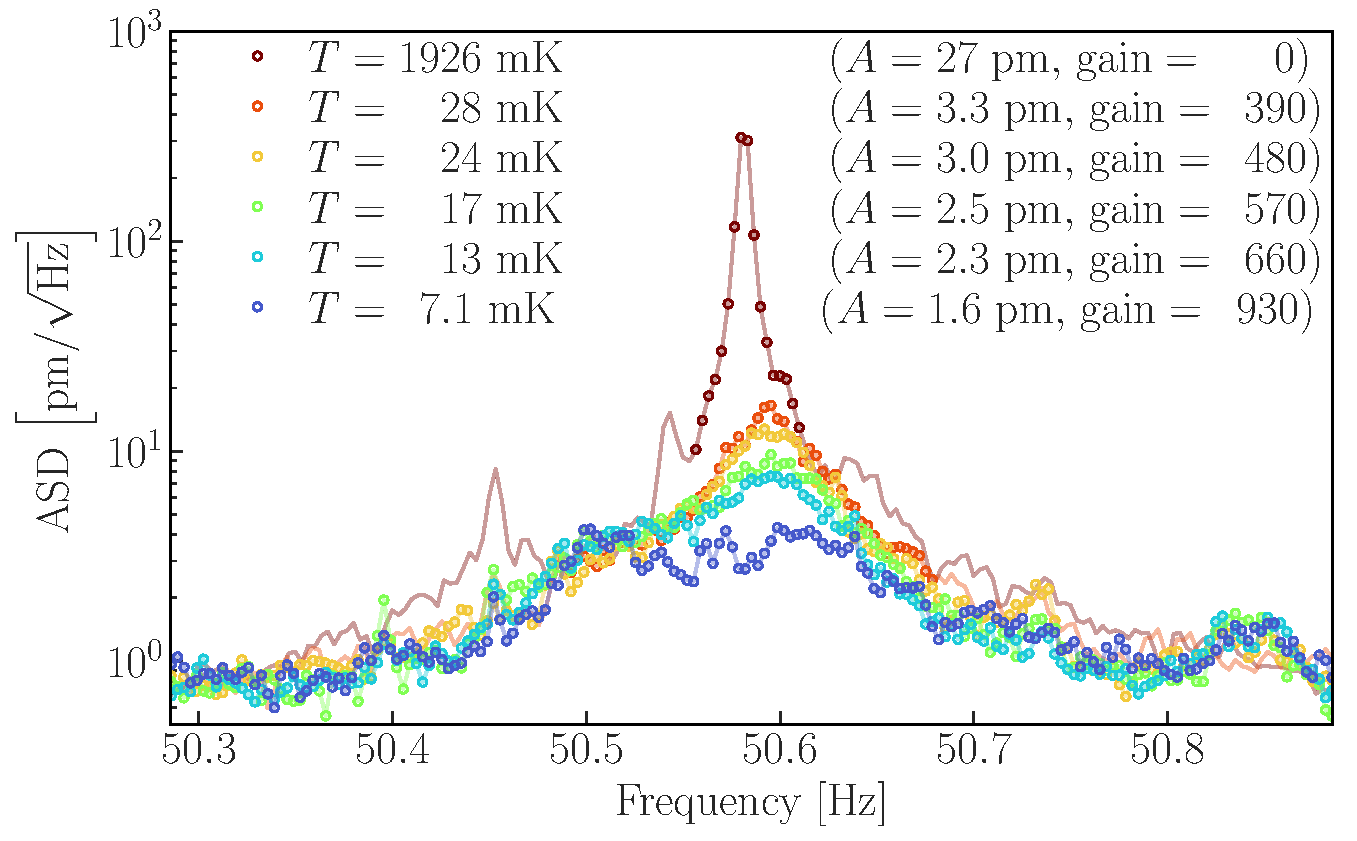
\includegraphics[width=\columnwidth]{Figures/paper_figure_mode_3.pdf}
    \caption{The linear feedback cooling on mode 3 is plotted. The different colored lines represent spectra taken with different linear gains. The legend shows the achieved mode temperatures with corresponding RMS amplitude and proportional gain values. Equal colors in this plot and in Fig.~\ref{fig:cooling4} indicate measurements are taken simultaneously.}
    \label{fig:cooling3}
\end{figure}

%\DU{Bas had bedacht om in deze twee figuren weer mode en RMS als subscript bij te zetten. Als we zouden wisselen naar de gamma FB notatie past dat wellicht wel. Louisa merkt op dat de gain nu geen betekenis heeft. Dat we beter naar dB of naar Gamma FB kunnen wisselen. Ik vind dat ze wel een punt heeft alleen dat we dat nu niet makkelijk kunnen doen toch?}\\
%\DU{Een andere suggestie van Bas is om het hier als $\sqrt{S_x} [pm/\sqrt{Hz}]$ te doen en in Fig. 2 wel als PSD. Wat vinden jullie? Ik heb zelf geen mega sterke mening los van dat ik dit even duidelijk vind als het andere}

Mode 4 has a resonance frequency of \SI{67.98}{Hz} and a Q factor of \SI{5.5e6}{}. The same cooling mechanism is applied to mode 4, in this case the lowest observed mode temperature is \SI{6.6}{mK} simultaneously with the \SI{7.1}{mK} of mode 3. Here, a gain of \SI{1500}{} is used and a corresponding RMS amplitude of \SI{1.2}{pm} is measured.

Both plots show lines and dots, the lines represent the measured data. The part of the data that falls within the mentioned bandwidth ($\text{BW}$) of $\left[ f_0-3f_0/Q, f_0+3f_0/Q \right]$ is visualised with the dots in both Fig.~\ref{fig:cooling3} and Fig.~\ref{fig:cooling4}. The shown RMS amplitude and mode temperature are therefore based on the cumulative sum of these dots. 

\begin{figure}[h]
    \centering
    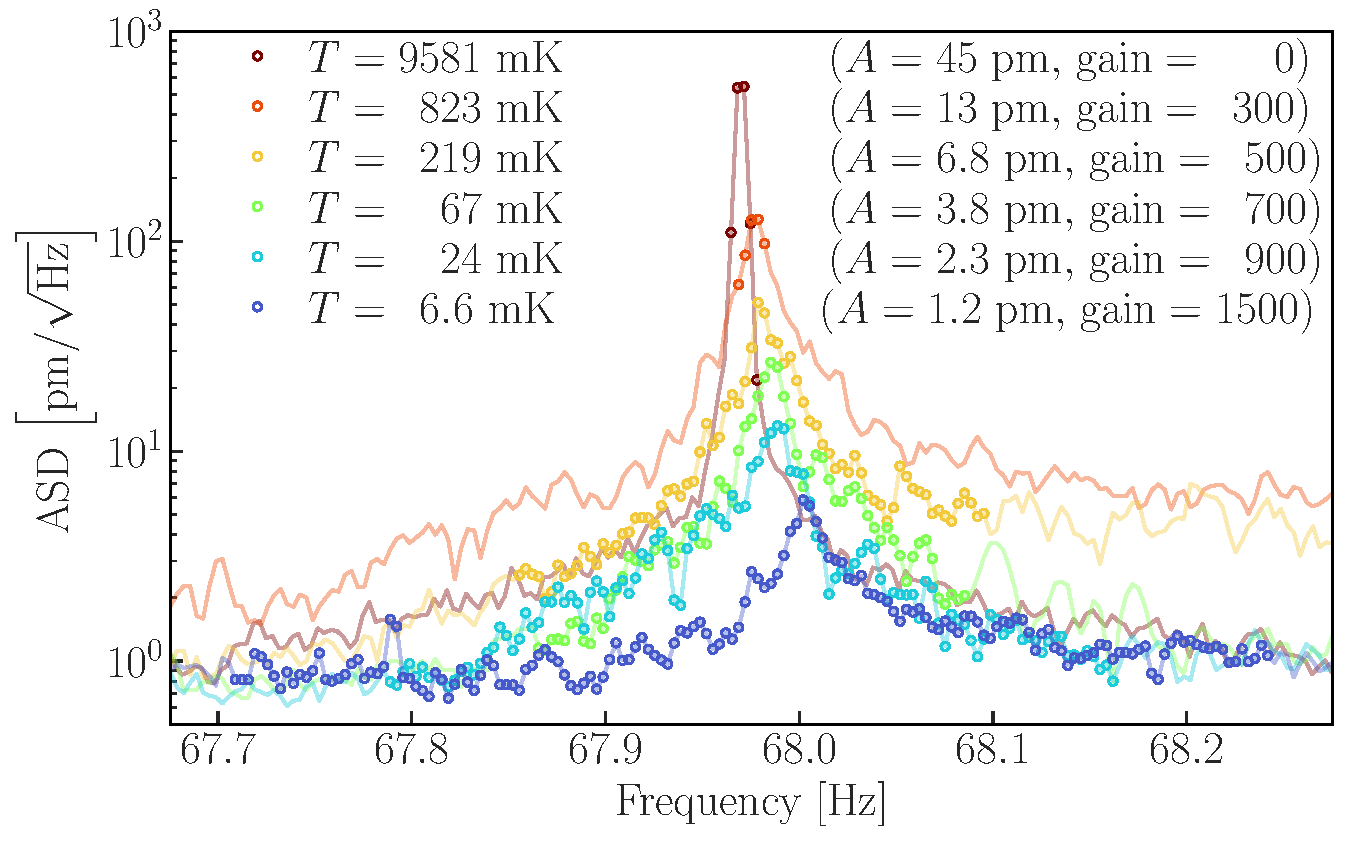
\includegraphics[width=\columnwidth]{Figures/paper_figure_mode_4.pdf}
    \caption{Similar to Fig.~\ref{fig:cooling3}, the linear feedback cooling on mode 4 is plotted. The different colored lines represent spectra taken with different linear gains. The legend shows the achieved mode temperatures with corresponding RMS amplitude and proportional gain values. Equal colors in this plot and in Fig.~\ref{fig:cooling3} indicate measurements are taken simultaneously.}
    \label{fig:cooling4}
\end{figure}

These results are achieved while not only doing active feedback on mode 3 and 4, but also on some of the mass spring system modes and on mode 2 with a second piezo. Active feedback is applied on these frequencies continuously to ensure a relatively quiet environment for the linear feedback on mode 3 and 4. During these measurements upconversion of noise peaks surrounding the resonance peaks is visible in the spectrum, see supplementary material~\ref{sec:mode mixing} for further details.

Mode temperature can be converted to a phonon number ($N_\text{ph}$) via:

\begin{equation}
    N_\text{ph} = \frac{k_B T_\text{mode}}{\hbar \omega_0}.
\end{equation}

In the case of mode 3 the lowest mode temperature corresponds to a value of $N_\text{ph, 3} = \SI{2.9e6}{}$ and for mode 4 a value of $N_\text{ph, 4} = \SI{2.0e6}{}$.

